\documentclass[10pt,a4paper]{article}
\usepackage[utf8]{inputenc}
\usepackage[T1]{fontenc}
\usepackage[left=2.00cm, right=2.00cm, top=3.00cm, bottom=3.00cm]{geometry}
\usepackage{abstract}
\usepackage{tikz}
\usepackage{url,hyperref}
\usetikzlibrary{arrows.meta, automata, shapes, arrows, calc, positioning, quotes}
\tikzstyle{dfa} = [rectangle, rounded corners, minimum width=3cm, minimum height=1cm,text centered, text=white, fill=blue!100, text width = 6.5cm]
\tikzstyle{nn} = [rectangle,  rounded corners, minimum width=3cm, minimum height=1cm,text centered, text=white, fill=red!100, text width = 6cm]
\tikzstyle{process} = [trapezium, trapezium left angle=70, trapezium right angle=110, minimum width=3cm, minimum height=0.5cm, text centered, draw=black, fill=gray!30, inner xsep=0pt,outer sep=0pt]
\tikzstyle{comparison} = [diamond, text centered, draw=black, fill=green!50, /pgf/aspect=1.3]
\tikzset{
	FARROW/.style={line width=2pt, arrows={-Latex[angle=40:4mm]}}
}
\tikzstyle{arrow} = [thick,->,>=stealth]

\title{Learning from Each Other: Neural Networks and Finite Automata \\
	{
		\large Networking Grant
	}
}
\author{Fredrik Dahlqvist}
\date{}

\begin{document}
	
	\maketitle
	
	\begin{abstract}
		\textbf{Abstract:}
		This project will explore how two machine learning paradigms -- \emph{finite automata} and \emph{neural network}  -- can improve and explain each other. It consists of two tracks. 
		
		The first, led by QMUL, will use finite automata to understand \emph{compositionality} and \emph{modularity} in neural networks. Finite automata form a rich suite of classification problems that can be combined in several ways. Using this feature, we will compare how a neural network solves a combination of two problems with how it solves the individual problems. This should reveal the mechanisms of modularity in neural networks, a key step towards explainable AI.
		
		The second track, led by Cornell, will use neural networks to improve the state-of-the-art algorithm for learning finite automata. This task has many industrial applications but faces a computational bottleneck consisting of \emph{generating} certain counterexamples. We will use generative AI, i.e.\ specialist neural networks, to solve this problem.
		\\
		\\
		\textit{\textbf{Keywords:} Machine learning, finite automata, neural network, explainable AI}
	\end{abstract}
	
	\section{Quality and relevance}
	
		This project aims to explore how two well-known machine learning paradigms -- \emph{finite automata} and \emph{neural network} learning -- can help improve and explain each other. The primary deliverable of this exploration will be the development of a joint Cornell-QMUL grant proposal on the topic. In the process we hope to generate some early results and prototypes.
		
		Concretely, this project is structured around two research tracks which aim to create flows of knowledge from Cornell to QMUL and from QMUL to Cornell, echoing the technical objective of creating flows of knowledge from finite automata learning to neural network learning and vice-versa. The title of the project --  \emph{Learning from Each Other} -- therefore refers to the  twin objectives that both human and algorithmic learners will learn from each other. 
		
		Based on the expertise and research interests of the two PIs and their collaborators, Cornell will be the finite automata pole of this research program, and QMUL will be the neural network pole. The project will leverage the expertise of each pole to help solve problems faced by the other. 
	
		{
				\vspace{3mm}
				\noindent \textsc{\large a) Improving our understanding of Neural Networks with Finite Automata}
				\vspace{3mm}
		}
	
		The first problem, led by the QMUL half of the project, is to make progress on understanding how \emph{Neural Networks}, the main technology behind the current generative AI revolution, actually work. Explainable AI is a very active field of research but much remains mysterious about neural networks. How can we explain their incredible effectiveness versus other models of computation? Is it possible to understand how a neural network works -- and therefore also how it doesn't -- in a structural and compositional way, that is to say by understanding it as a composition of smaller and better understood sub-systems? Since these models find applications in virtually every industry, and will more or less directly impact everyone on the planet, these are societally crucial problems. 
		
		To investigate these questions we propose to use the expertise of the Cornell pole in the theory and industrial applications of \emph{finite automata}, one of the simplest and best-understood models of computations. A finite automaton represents a simple `computing machine' which can only successfully run programs written in a simple `programming language' called a regular expression. An automaton can thus be used to solve the problem of deciding whether a program belongs to such a language or not: simply feed the program to the automaton and check whether executes successfully or not. Neural networks can also solve this classification problem, and our proposal is therefore to use finite automata as a well-understood, well-behaved and sufficiently complex benchmarking and testing suite with which to probe the inner workings of neural networks. 
	
		
		This is not a new idea, \cite{cleeremans1989finite} provides a brief but very instructive example of this line of research from a natural language processing perspective. Much of the research at the intersection between neural network and finite automata has since focused on describing the behaviour of an unknown neural network as a finite automaton \cite{weiss2018extracting,weiss2019learning} or using automata theory to describe the computational power of neural networks \cite{weiss2018practical}. Our proposed approach combines the original idea of~\cite{cleeremans1989finite} -- trying to understand how a neural network works by discovering how it internally represents the finite automaton problem it is solving -- to the more recent work of \cite{weiss2018extracting,weiss2019learning} which which gives concrete algorithms to extract this internal representation. This will allow us to perform the following type of neural network probing experiment: (a) set an automaton problem, (b) solve it with a neural network, (c) extract the network's internal representation of the automaton, and (d) compare it to the original, as described in Figure \ref{diag:strategy}. 
		
		Finite automata form a space of problems with a rich inner structure, for example automata $A$ and $B$ can be combined in various ways to form new automata, say $A+B$. Using the strategy of Figure~\ref{diag:strategy} we can study the compositional nature of neural networks by understanding how the internal representations of $A$ and $B$ are combined to form an internal representation of $A+B$ in the neural network. We will also investigate whether a new neural network pruning procedure developed at QMUL~\cite{pruning} in order to optimally compress neural networks, can be used to improve the Automaton Learning part of this strategy.	
		
	
		\begin{figure}[ht]
			\begin{center}
				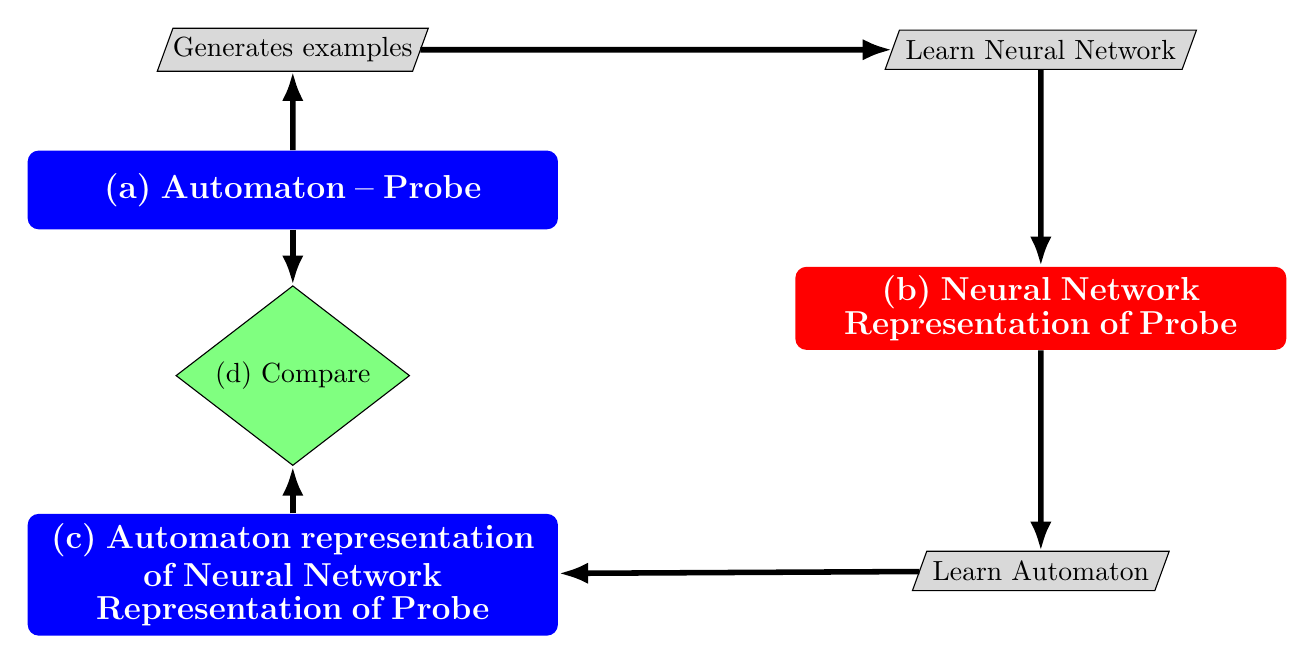
\begin{tikzpicture}[node distance=9.5cm]
					\node (start) [dfa] {\large \bf (a) Automaton -- Probe};
					\node (examples) [process, above = 1cm of start] {Generates examples};
					\node (learn1) [process, right of = examples] {Learn Neural Network};
					\node (step2) [nn, below= 2.5cm of learn1] {\large \bf (b) Neural Network \\ Representation of Probe};
					\node (end) [dfa, below = 3.6cm of start] {\large \bf  (c) Automaton representation \\ of Neural Network \\ Representation of Probe};
					\node (learn2) [process, below = 2.55 of step2] {Learn Automaton};
					\node (compare) [comparison, above = 0.6cm of end] {(d) Compare};
					\draw [FARROW] (start) -- (examples);
					\draw [FARROW] (examples) -- (learn1);
					\draw [FARROW] (learn1) -- (step2);
					\draw [FARROW] (step2) -- (learn2);
					\draw [FARROW] (learn2) -- (end);
					\draw [FARROW] (end) -- (compare);
					\draw [FARROW] (start) -- (compare);
				\end{tikzpicture}
			\end{center}
			\caption{Learning and testing strategy}
			\label{diag:strategy}
		\end{figure}
	
		
		{
			\vspace{3mm}
			\noindent \textsc{\large b) Learning Finite Automata with the help of a Neural Network}
			\vspace{3mm}
		}
	
		As mentioned above, finite automata solve the problem of identifying which `programs' are written in the `programming language' described by a so-called regular expression. In 1987 Dana Angluin~\cite{angluin1987learning} developed a famous  algorithm which showed that it is possible to \emph{learn} an \emph{unknown} automaton by $(i)$ feeding it programs and observing whether they run successfully or not (these interactions are called membership queries), and $(ii)$ asking for a counter-example program that runs successfully on the algorithm's current representation of the unknown automaton, but not on the actual unknown automaton (these interactions are called equivalence queries).  The Cornell pole has unrivalled expertise in applying and extending this algorithm to an extremely wide variety of applications.
	
		A major practical obstacle in Angluin's algorithm is that of implementing equivalence queries since, by definition, the target automaton is unknown. Counter-examples are typically generated by exhaustive testing, which is highly resource and time-intensive. To solve this problem, we propose that the  QMUL pole develop and train neural networks to generate counter-examples in Angluin's learning algorithm. This approach aims to exploit the strength of generative AI,  by training specific neural network architectures like GANs (generative adversarial networks) or LLMs (Large Languages Models) on the programs which fail membership queries, thereby learning to generate candidate counter-example programs.
		
		 {
		 	\vspace{3mm}
		 	\noindent \textsc{\large c) The Team}
		 	\vspace{3mm}
		 }
	
		\begin{itemize}
			\item QMUL pole
				\begin{itemize}
					\item \textbf{PI}: Dr.\ Fredrik Dahlqvist is a lecturer at QMUL whose research focuses on programming languages and formal methods in the context of machine learning, specifically probabilistic programming languages. Prior to joining QMUL Fredrik was a senior researcher at UCL working with Prof.\ Silva. This proposal aims to provide the means to preserve and extend this successful existing working relationship.
					\item \textbf{co-I}: Gabryel Thomas-Mason is a PhD student at Queen Mary University of London and a Google Scholarship recipient. Gabryel's PhD focuses on the interpretability and efficiency of deep learning models. In addition, Gabryel is a research software engineer at the Rosalind Franklin Institute, conducting research into novel approaches to High-performance computing, cloud, data compression and storage. 
				\end{itemize}
			\item Cornell pole 
				\begin{itemize}
					\item \textbf{PI} Prof.\ Alexandra Silva 
					\item \textbf{co-I}: ? Tiago?
				\end{itemize}
		\end{itemize}
	
	
	\section{Execution and sustainability}
	
		As mentioned above, the main deliverable of this project will be the development of a joint Cornell-QMUL grant proposal. We plan to target joint US-UK funding programs, in particular the well-established NSF-EPSRC collaborations. This could be done either through a NSF grant under e.g.\ the \emph{Computing and Communication Foundations -- Algorithmic Foundations} or the \emph{Information and Intelligent Systems -- Robust Intelligence}\footnote{(\url{https://www.nsf.gov/od/oise/IntlCollaborations/UK.jsp}} programs, or through an EPSRC \emph{Working with Overseas Scientists} grant \footnote{\url{https://www.ukri.org/opportunity/epsrc-working-with-overseas-scientists-nov-2023-responsive-mode/}}. Alternatively, the project we have in mind fits very well with ARIA's \emph{Safeguarded AI} program\footnote{\url{https://www.aria.org.uk/programme-safeguarded-ai/}}. We aim to have the proposal ready for submission by the end of 2025. In order to meet this target we have allocated funding for one trip by the QMUL PI to Cornell and one trip from the Cornell PI to London (1-2 weeks each).
		
		In the process of developing this grant proposal we expect to generate some early results and prototypes which we plan to present at workshops. For example, early result on Track B) -- Learning Finite Automata with the help of a Neural Network -- could be presented at LearnAut, the workshop dedicated to automata learning in the course of 2025.  Similarly, early results on Track A) could be presented at one of the many workshops colocated with the large machine learning conferences like NeurIPS or ICLR. This has been costed in the attached budget by adding a workshop visit for both poles the project. \emph{Perhaps sell this as an opportunity for the co-I(s)/more junior members to present early work?}
	
		
	\section{Impact}
		As an early career, recently appointed academic, Fredrik Dahlqvist would benefit immensely from a successful grant proposal, particularly in collaboration with such an experienced researched as Prof.\ Silva. The proposed research would also help him turn an initial research foray in the sphere of machine learning -- which led to the publication of \cite{pruning} at the prestigious ICLR conference with the QMUL co-I -- into a more established presence in the field.
		
		Alex?
		
		This project can be understood as a multi-disciplinary effort, which aims to connect and cross-fertilize two fields (neural networks and finite automata) which exist in largely disjoint ecosystems. At a very high level of description, the impact of the proposed research should therefore be to enrich each of these fields with techniques and ideas from the other, in the spirit of the title of the project -\emph{Learning from Each Other}. 
		
		More concretely, any improvement in Angluin's famous algorithm will have a direct on its applications in industry .... \textit{ask Alex about this!} 
		On the neural network side, the societal impacts of this technology are so enormous, that even modest new insights into compositionality, modularity and explainability of neural networks can have a potentially huge impact. The proposed research is based on an entirely new yet computationally realistic methodology for probing the compositional nature of neural networks based on solid theoretical foundations. We are therefore confident that some completely new mechanisms and properties of neural networks can be revealed. 

	
	
	\bibliographystyle{plain}
	\bibliography{proposal}
\end{document}